% Intended LaTeX compiler: pdflatex
\documentclass[a4paper,12pt]{article}
                \usepackage[mathletters]{ucs}
                \usepackage[utf8x]{inputenc}
                \usepackage{sectsty}
                \sectionfont{\normalfont\scshape}
                \subsectionfont{\normalfont\itshape}
                \usepackage[round,authoryear]{natbib}
                \usepackage{amsmath}
                \newtheorem{theorem}{Theorem}
                \newtheorem{assumption}{Assumption}
                \newtheorem{acknowledgement}{Acknowledgement}
                \newtheorem{algorithm}{Algorithm}
                \newtheorem{axiom}{Axiom}
                \newtheorem{case}{Case}
                \newtheorem{claim}{Claim}
                \newtheorem{conclusion}{Conclusion}
                \newtheorem{condition}{Condition}
                \newtheorem{conjecture}{Conjecture}
                \newtheorem{corollary}{Corollary}
                \newtheorem{criterion}{Criterion}
                \newtheorem{definition}{Definition}
                \newtheorem{example}{Example}
                \newtheorem{exercise}{Exercise}
                \newtheorem{lemma}{Lemma}
                \newtheorem{notation}{Notation}
                \newtheorem{observation}{Observation}
                \newtheorem{problem}{Problem}
                \newtheorem{proposition}{Proposition}
                \newtheorem{remark}{Remark}
                \newtheorem{result}{Result}
                \newtheorem{summary}{Summary}
                \newtheorem{Hypothesis}{Hypothesis}
                \newcommand{\qed}{\hspace*{\fill} {\em Q.E.D.}}
                \usepackage{pdftexcmds}
                \usepackage{textcomp}
                \usepackage{hyperref}
                \usepackage{graphicx}
                \usepackage{mathtools}
                \mathtoolsset{showonlyrefs=true}
                \linespread{1.3}
                \usepackage[right=3cm, left=3cm,top=3cm,bottom=3cm]{geometry}
               \usepackage{listings}
               \makeatletter
\newcommand{\citeprocitem}[2]{\hyper@linkstart{cite}{citeproc_bib_item_#1}#2\hyper@linkend}
\makeatother
\usepackage[round,authoryear]{natbib}
\setcitestyle{authoryear, round, comma, aysep={;}, yysep={,}, notesep={, }}
\author{Jan Boone\thanks{Tilburg University, Department of Economics, Tilec and CEPR, E-mail: \textit{j.boone@uvt.nl}.}}

\setcounter{secnumdepth}{2}
\date{\today}
\title{Pricing above value: selling \emph{to} a market with selection problems}
\hypersetup{
 pdfauthor={},
 pdftitle={Pricing above value: selling \emph{to} a market with selection problems},
 pdfkeywords={},
 pdfsubject={},
 pdfcreator={Emacs 29.2 (Org mode 9.7-pre)}, 
 pdflang={English}}
\begin{document}

\maketitle
\maketitle
\begin{abstract}
This paper shows that selection incentives in downstream markets distort upstream prices. It is possible for inputs to be priced above the value that the good has for final consumers. We apply this idea to pharmaceutical companies selling drugs to a health insurance market with selection problems. We specify the conditions under which drugs are sold at prices exceeding treatment value. Another feature of the model is an excessive private incentive to reduce market size, e.g. in the form of personalized medicine.
\end{abstract}

\textbf{Keywords:} selection, pricing above value, vertical relations, pharmaceutical prices

\textbf{JEL codes:} I13, I11


\newpage

\section{Introduction}
\label{sec:org508124e}

With some regularity there appear newspaper articles documenting the level and increases in drug prices. Experts argue that some patented drugs are priced above their value for patients. From an economic point of view this seems impossible: if the price of a treatment exceeds its value for consumers, a health insurer should not cover this treatment in its contracts. This paper introduces a model that shows that, in fact, it can be optimal for an insurer to cover such a treatment and hence that it is optimal for a pharmaceutical company to price its drug above patient value. The key insight is that health insurance is a selection market and pharmaceutical companies sell to this market. The selection problems in the downstream (insurance) market distort prices in the upstream (pharmaceutical) market.

Examples of newspaper stories on pharmaceutical companies charging ``outrageous'' prices for their treatments include \url{https://nyti.ms/2NvLoZx}, \url{https://nyti.ms/2bHXkFj} and \url{https://nyti.ms/2nKMJ2a}.\footnote{Although the links are ``clickable'' in the pdf version of the paper, navigation is easier in the html version at: \href{https://janboone.github.io/Treatment-Prices/}{https://janboone.github.io/Treatment-Prices/}. This webappendix includes details of the model underlying Figure \ref{fig:profitfunctions}.} Although it is hard to put a value on an additional year of life to see whether prices are above treatment value, for anticancer drugs ``in 1995 patients and their insurers paid \$54,100 for a year of life. A decade later, 2005, they paid \$139,100 for the same benefit. By 2013, they were paying \$207,000'' (\citeprocitem{23}{Howard et al. 2015, 149}). Most regulators in the world use less than \$200k as the monetary value of a life year and indeed at the World Oncology Forum the ``prevailing opinion was that \ldots{} the cost of the new generation of drugs is getting out of all proportion to the added benefit'' (\citeprocitem{4}{Cavalli 2013}).

Further, it has been noted that ``prices of \ldots{} drugs in the so-called `specialty' pharmaceutical market have been increasing over time'' (\citeprocitem{23}{Howard et al. 2015, 140}). The promise of specialty or precision medicine was ``to give `the right drug to the right patient' to maximize the effectiveness and safety of the treatment'' (\citeprocitem{16}{Garattini, Curto, and Freemantle 2015}). However, up till now this targeting of treatments has not lived up to this promise and one reason is that these treatments turn out to be extremely expensive. It is not clear that we can afford precision medicine. To illustrate, in oncology there are treatments costing \$300,000 while they ``only result in minimal benefit'' (\citeprocitem{10}{Doble 2016}).

To analyze whether it is possible for drugs to be priced above their value for patients, we introduce a model with upstream pharmaceutical companies selling drugs to downstream insurers for inclusion in their health insurance contracts. The health insurance market suffers from selection. The condition we need for our results is that low risk types are tempted to buy the insurance contract aimed at high risk types. This can happen if high risk types feature a higher elasticity on the health insurance market than low risk types. Pharmaceutical firms then charge prices in excess of their treatments' value for patients and still have their treatments covered by insurance. To increase the premium for low risk contracts, insurers distort the high type's allocation upwards by covering a treatment that is expensive. 

Moreover, targeting of pharmaceutical R\&D investments on subgroups (precision medicine) tends to increase the gap between price and patient value further. This result sheds light on developments in specialty drugs or personalized medicine where higher prices are easier to spot than improved treatments. Finally, the introduction of generic drugs helps to increase prices of patented drugs. To the extent that people can decide to go without insurance, the insurance premium cannot exceed the total value of the insurance contract. Generic drug competition leads to prices below the value of treatment thereby creating the ``space'' for patented drugs to charge prices above value.

In the next section we discuss the empirical evidence that supports the assumption that low risk types want to buy the generous high risk type contract. Further, our analysis is related to the following strands of literature. 

First, there are a number of explanations for high drug prices found in the literature (\citeprocitem{23}{Howard et al. 2015}). However,  these cannot fully explain why prices would exceed treatment value. To illustrate, an explanation that is often mentioned is that with health insurance people want a treatment, no matter what the cost since the insurer pays (most of) the price. This is true ex post: once I have insurance, the effects of the cost of treatment are reduced for me. Economists tend to refer to this as moral hazard. However, why would I buy insurance coverage for a treatment that costs more than the benefit it provides? Dropping such a treatment from the contract leads to a bigger reduction in the premium than the loss in expected utility. Hence, an insurer --whether or not it has market power-- benefits from removing such treatments from its insurance contract. This threat of not being covered by an insurance contract limits the price a pharmaceutical company can ask for patented drugs.

Similarly, high sunk costs of R\&D are often mentioned to explain high treatment prices (\citeprocitem{17}{Garrison and Towse 2017}). Although high fixed/sunk costs can explain high prices in competitive markets (by limiting entry), this mechanism is not obvious for a monopoly market where a firm is protected by a patent. Since a monopolist tries to appropriate most or all of the surplus from its customers, its sunk fixed costs are not directly relevant for setting prices. And also here, if the treatment is too expensive, it should be dropped by the insurer from the contract.\footnote{In free market systems, the insurer can decide what to cover or not in its contracts. In regulated market systems, like the Netherlands, the government often prescribes which conditions need to be covered by basic insurance but does not define which treatments need to be covered.}

Other papers focus on the relation between prices and disease rarity: the lower the prevalence of a disease, the higher the prices for drugs treating it. In the context of orphan drugs, this is sometimes referred to as payers valuing rarity (\citeprocitem{29}{Medic et al. 2017}; \citeprocitem{30}{Messori, Cicchetti, and Patregani 2010}). If the insurance premium is determined by the budget constraint of the marginal insured, an inverse relation exists between disease prevalence and drug price (\citeprocitem{25}{Kamphorst and Karamychev 2021}). We offer a complementary explanation for this inverse relation via the selection incentives on the health insurance market.

In terms of the mechanism design literature, our focus on a binding incentive compatibility constraint for low types is in line with the countervailing incentives literature (\citeprocitem{27}{Lewis and Sappington 1989}). This literature considers type dependent outside options, which we generate through differing demand elasticities for different types. Although we use health insurance and selection to illustrate our model, the mechanism applies in any screening model where the incentive compatibility constraint is binding for the low type.

In (health) insurance markets this situation with binding incentive compatibility constraints for low types is reminiscent of advantageous selection (\citeprocitem{12}{Einav and Finkelstein 2011}; \citeprocitem{28}{Mahoney and Weyl 2017}). There are two main differences between these papers and our model. First, we allow insurers to screen consumers into different contracts instead of each firm offering only one contract. Second, we analyze the effects of selection on upstream prices. 

Our paper is organized as follows. The next section introduces a simple model with imperfect competition in the health insurance market. We discuss our assumption that low risk types want to mimic high risk types. Then we derive our main result that pharmaceutical companies selling to this health insurance market can charge prices above the value of their treatments. We analyze the incentives to target treatments at sub-groups (precision medicine) and conclude with a discussion of policy implications.

\section{Simple model}
\label{sec:example}
\label{sec:example}

To see how it is possible that an insurer pays more for a treatment than the treatment's value to the insured, consider the following model with two treatments and (imperfectly) competing insurers. 

Denote the two treatments 1 and 2; both treatments are produced at marginal costs normalized to zero: \(c_1 = c_2 =0\). Treatment 1 is under patent. Treatment 2 is off patent and sold by competing generic drug producers at a price equal to marginal costs. The values of these treatments are given by \(v_1,v_2\) resp. and are the same for each patient. Value \(v_i\) captures things like life years gained, increased utility due to improved quality of life, increased productivity etc. (\citeprocitem{17}{Garrison and Towse 2017}). Although it is not straightforward to measure this in practice, conceptually the value of a treatment is well defined. We aim to show that pharmaceutical companies can profitably charge a price in excess of this value and still be covered by insurance plans.


Competing insurers sell insurance to a customer who can be either of risk type \(l\) (probability \(\phi\)) or type \(h\) (probability \(1-\phi\)). Type \(k=l,h\) needs treatments 1,2 with probability \(\psi_{1k},\psi_{2k} \in \langle 0,1]\). We assume single crossing: \(\psi_{ih} \geq \psi_{il}\) for \(i=1,2\). To simplify notation, we assume that \(\psi_{2h} = \psi_{2l} = \psi_2\).\footnote{Our working paper version generalizes the model and the results below to sets of patented and generic drugs with type dependent values for all \(\psi\)'s.} The high risk consumer has a strictly higher probability of needing treatment 1: \(\psi_{1h}>\psi_{1l}\). Thus the insurer's expected costs are higher for type \(h\) than for type \(l\) as \(h\) is more likely to need treatment.

We assume that the consumer buys insurance to get access to treatments. That is, without insurance, the consumer goes without treatment.\footnote{To simplify notation, we normalized \(c_1=c_2=0\). For the access to care interpretation, think of \(c_1,c_2\) being high enough that a patient without insurance cannot afford them even at cost price.} This has two reasons. First, it is well documented that people without health insurance tend to forgo treatment as they have difficulty financing it. These access issues have been stressed both in the popular press (\citeprocitem{7}{Cohn 2007}) and in academic journals (\citeprocitem{32}{Nyman 1999}; \citeprocitem{37}{Schoen et al. 2008}; \citeprocitem{38}{Schoen et al. 2010}). Many governments are concerned about health consumption inequality caused by income differences and design policies to make healthcare accessible to low income families (\citeprocitem{39}{Schokkaert and van de Voorde 2011}).

Second, it streamlines the analysis. With risk aversion as motivation to buy insurance, we need a non-linear (concave) utility function. Further, with risk aversion there is an additional reason why insurers prefer high prices for treatments: it is more attractive for customers to insure an expensive treatment than a cheap one. Both effects make derivations less straightforward while not changing our results.\footnote{The appendix introduces a model with only risk aversion to illustrate the difference with our selection framework.}

Each insurer offers two contracts (which can be identical in case of a pooling outcome), each contract aimed at a consumer type. We write the value/utility of the contract for type \(k=1,2\) as follows:
\begin{equation}
\label{eq:5}
u_{k} = \psi_{1k} x_{1k} v_1 + \psi_{2} x_{2k} v_2 - \sigma_k
\end{equation}
where \(x_{ik} \in [0,1]\) denotes the probability that treatment \(i\) is covered by contract \(k\) (below we have that \(x_{ik}\) equals either 0 or 1) and \(\sigma_k\) denotes the price/premium of contract \(k\). Value \(v_i\) denotes the utility of receiving the treatment in case the consumer needs it (with probability \(\psi_{ik}\)) compared to not receiving this treatment. Note that falling ill in itself can cause a disutility for the individual. Taking this into account would add a constant to the expression in \eqref{eq:5} which we leave out to ease notation.

The incentive compatibility (IC) constraints for these contracts can be written as follows.

\begin{equation}
\label{eq:2}
u_h \geq  \psi_{1h} x_{1l} v_1 + \psi_{2} x_{2l} v_2 - \sigma_{l}
\end{equation}
\begin{equation}
\label{eq:4}
u_l \geq  \psi_{1l} x_{1h} v_1 + \psi_{2} x_{2h} v_2 - \sigma_h
\end{equation}
The first equation, \(IC_h\), implies that the high type is better off choosing the high contract (yielding utility \(u_h\)) than to buy the low type's contract (which yields her utility equal to the right hand side of \eqref{eq:2}). To illustrate, the \(h\) type needs treatment 1 with probability \(\psi_{1h}\), but the \(l\) contract provides this treatment with probability \(x_{1l}\) in which case she gets utility \(v_{1}\); the price of this contract equals \(\sigma_{l}\). And, similarly, \(IC_l\) implies that the low type is better off buying the \(l\) contract --yielding \(u_l\) -- than buying the \(h\) contract which yields her utility equal to the right hand side of \eqref{eq:4}. These constraints capture intra-brand competition faced by the insurer: if the \(h\) contract becomes too attractive, \(l\) types buy this contract instead of the \(l\) contract (that is, \eqref{eq:4} is violated).

As we will see below, pricing a treatment above its value is possible if low types want to mimic high types; that is, \(IC_l\) is binding. The next section shows that this can happen when the \(h\) market is more elastic than the \(l\) market.

\subsection{First best}
\label{sec:org277164b}

A straightforward way to check which incentive constraint is binding in second best is to derive the first best outcome. First best is defined here as the case where insurers can observe insured's risk type and are allowed to risk rate. Put differently, first best here refers to the absence of asymmetric information.

The profit an insurer makes on type \(k\) is given by \(\sigma_k - \psi_{1k}x_{1k}p_1 - \psi_{2}x_{2k}p_2\): insurance premium minus expected costs for type \(k\) where insurers' costs are determined by the prices \(p_{i}\) charged by the pharmaceutical companies. Solving equation \eqref{eq:5} for \(\sigma_{k}\) and substituting this into the expression for the per type profit gives:
\begin{equation}
\label{eq:6}
\pi_k = \psi_{1k}x_{1k}(v_1-p_1)+\psi_{2}x_{2k}(v_2-p_2)-u_k
\end{equation}
and the insurer's overall profits are given by
\begin{equation}
\label{eq:7}
\Pi = \phi q_l(u_l) \pi_l +(1-\phi)q_h(u_h) \pi_h
\end{equation}
In words, the fraction \(\phi\) of low types times the insurer's market share \(q_l\) on the \(l\) market --which depends on the utility \(u_l\) offered to the \(l\) type-- 
times the per customer profit \(\pi_l\) on the \(l\) market; and similarly for the \(h\) market segment. We assume that the insurer's market share on the \(k\) segment, \(q_k\), is increasing in the utility offered to type \(k\), \(q_k'(u_k)>0\) for \(k=l,h\). 

With \(p_1=v_1\) and \(p_2=0\) due to competition on the generic (off-patent) market, we write an insurer's optimization problem as:
\begin{equation}
\max \phi q_l(u_l) (\psi_2 x_{2l} v_2 -u_l) + (1-\phi) q_h(u_h) (\psi_2 x_{2h} v_2 -u_h)
\end{equation}
The first order condition for \(u_k\) (\(k=l,h\)) can be written as
\begin{equation}
\frac{\partial q_{k}}{\partial u_{k}} (\psi_2 x_{2k} v_2 - u_k) - q_k = 0
\end{equation}
It is routine to verify that this can be written as
\begin{equation}
\label{eq:elastEquation}
u_k = \frac{\varepsilon_{k}}{1+\varepsilon_{k}}\psi_2 v_2
\end{equation}
where the elasticity is defined as \(\varepsilon_k = \partial q_k/\partial u_k * u_k/q_k\): the percentage increase in demand in response to a one percent increase in utility offered to market segment \(k\). The next section discusses what this elasticity captures and how it can differ between risk types.

We are interested in the case where \(IC_h\) is satisfied and \(IC_l\) is violated. This happens when inequality \eqref{eq:4} is violated. It is routine to verify that the violation of \eqref{eq:4} can be written as:
\begin{equation}
\label{eq:1}
u_l < \psi_{1l}x_{1h}v_1 + \psi_2x_{2h}v_2 -\sigma_h = u_h - (\psi_{1h}-\psi_{1l})x_{1h} v_1
\end{equation}
In first best it is optimal to cover treatment 1 (\(x_{1h}=1\)) as long as \(p_1 \leq v_1\). We write \(\Delta \psi_1 = \psi_{1h} - \psi_{1l}\). Hence, \(IC_l\) is violated in the first best outcome if
\begin{equation}
u_h - u_l > v_1 \Delta \psi_1
\end{equation}
Using \eqref{eq:elastEquation}, we can write this inequality as
\begin{equation}
\label{eq:ICelasticities}
\frac{\varepsilon_{h}}{1+\varepsilon_{h}} - \frac{\varepsilon_{l}}{1+\varepsilon_{l}} > \frac{v_{1} \Delta\psi_1}{\psi_2 v_2}
\end{equation}
In words, if the \(h\) market is sufficiently more elastic than the \(l\) market,\footnote{Note that \(\varepsilon/(1+\varepsilon)\) is increasing in \(\varepsilon\).} the first best solution violates the \(IC_l\) constraint (and satisfies \(IC_h\)). As we are working here with \(p_1=v_1\), the interpretation is that the elasticity difference (between \(h\) and \(l\)) should exceed the cost difference \(p_1 \Delta\psi_1\) by enough to satisfy \eqref{eq:ICelasticities}.

The equation also shows why we need imperfect competition in the health insurance market. With perfect competition (infinitely elastic demand at the firm level) in both markets the left hand side equals 0 (because \(\lim_{\varepsilon \rightarrow \infty} \varepsilon/(1+\varepsilon) = 1\)) and the inequality cannot be satisfied.

Note that equation \eqref{eq:ICelasticities} focuses on one particular parameter constellation. In general, there are other cases where, for instance, \(IC_h\) is binding or where no IC constraint is binding. As these cases are not relevant for the argument developed in the paper, they are not analyzed here.

\subsection{Why are high risk types more elastic?}
\label{sec:orgc542c4d}

Equation \eqref{eq:ICelasticities} shows that \(IC_l\) is binding in case the high risk segment is sufficiently more elastic than the low risk segment.

Broadly speaking there are two reasons why the high risk market is more elastic or more competitive than the low risk market. First, high risk types tend to have more experience with the healthcare system (think of the chronically ill) than low risk types. Hence, they understand health insurance contracts better and are able to make a better informed decision when confronted with competing contracts. For low risk types, these contracts are hard to relate to and they tend to make a less informed (more random) choice.

Second, high risk types tend to have lower incomes and hence are more price sensitive than low risk types.\footnote{The correlation between health status and income is well documented in the empirical health literature (\citeprocitem{15}{Frijters, Haisken-DeNew, and Shields 2005}; \citeprocitem{14}{Finkelstein and McGarry 2006}; \citeprocitem{19}{Gravelle and Sutton 2009}; \citeprocitem{31}{Munkin and Trivedi 2010}). Potential explanations for this correlation include the following. High income people are better educated and hence know the importance of healthy food, exercise etc. Healthy food options tend to be more expensive and therefore better affordable to high income people. Or (with causality running in the other direction) healthy people are more productive and therefore earn higher incomes.} For people on low income it pays to keep searching for a contract that is, say, 50 euros cheaper while people on high income may not be bothered to spend time on this.

The main reason mentioned why high risk people are expected to be less elastic is that they may worry that a new insurer will not accept them or will treat them worse than their current insurer does (``the devil you know\ldots{}''). Hence they are less likely to switch insurer in response to a better contract offered by a competing insurer. Underlying this idea is the notion that high risk types are loss making and hence insurers may not be willing to invest effort to keep them happy. There are two problems with this argument. First, as the model above shows, high risk types are profitable (and they would actually be more profitable if they were less elastic than the low risk types). Hence, there is no reason a priori why an insurer would try to get rid of them by treating them badly. Second, as we argue below, evidence found in earlier studies to show this lower elasticity for high types can be interpreted as evidence that high types are actually more elastic. 

The following papers present empirical evidence suggesting that high risk individuals are more sensitive to value differences between insurance contracts than low risk types. First, price elasticity is higher for people with a chronic condition (high risk) than without (\citeprocitem{33}{Parente, Feldman, and Christianson 2004}; \citeprocitem{5}{Chandra, Flack, and Obermeyer 2021}). Further, as high risks are better informed, they are more sensitive to quality differences between plans (\citeprocitem{18}{Gaynor, Ho, and Town 2015}). And there are papers documenting the idea that insurer switching probability falls with income and that the higher educated and the wealthier are less price sensitive (\citeprocitem{22}{Ho, Hogan, and Scott Morton 2017}; \citeprocitem{1}{Atherly, Dowd, and Feldman 2004}; \citeprocitem{2}{Auerbach and Ohri 2006}; \citeprocitem{36}{Saltzman 2019}; \citeprocitem{35}{Royalty and Solomon 1999}).

As mentioned, there are also papers suggesting that people with lower health status tend to be less price elastic when choosing insurance. These papers tend to be based on age as an indicator of health status: older people tend to have lower health status (\citeprocitem{40}{Strombom, Buchmueller, and Feldstein 2002}; \citeprocitem{35}{Royalty and Solomon 1999}). Others find no difference in elasticity between age groups (\citeprocitem{8}{Costa and Garcia 2003}).

One reason for the seemingly lower price elasticity is that people with low health status tend to be better informed about the quality of the different health plans and the treatments they cover. This can explain why they react less to price changes (they are more interested in quality than in price) and react less to plan quality information published by the government or an employer (\citeprocitem{3}{Beaulieu 2002}). They do not react to this newly published information because they know it already. Hence, the evidence showing a lower elasticity for high risk types can actually be interpreted as suggesting a higher elasticity for these types. 

Finally, as we show above, if the high risk segment is more elastic than the low risk segment, low risk types want to mimic high risk types (that is, \(IC_l\) is violated). Two recent papers document this behavior (\citeprocitem{21}{Handel and Kolstad 2015}; \citeprocitem{20}{Handel et al. 2020}).\footnote{One of the reasons why this happens is a deviation from rationality. The working paper version of our paper shows that bounded rationality can strengthen our results.} If it would be the case that the high risk segment is less elastic than the low risk segment, we should only observe high risk types buying low risk contracts.


\section{Pricing above value}
\label{sec:org62bd1a9}

The previous section showed that with the elasticity difference between high and low risk types compensating the cost difference, the incentive compatibility constraint for the low type (\(IC_l\)) tends to be binding. In this section we show how this allows a pharmaceutical company to charge a price that exceeds treatment value.

\subsection{Insurer's optimization problem}
\label{sec:orgf07c36f}

With \(IC_l\) binding, we write the insurer's profit maximization problem as follows; where we assume as before that \(p_1=v_1\) and \(p_2=0\).
\begin{align*}
\max_{u_l,u_h,x_{1l}, x_{1h},x_{2l},x_{2h}} & \phi q_{l}(u_l) (\psi_2 x_{2l} v_2 -u_l) + (1-\phi) q_h(u_h) (\psi_2 x_{2h} v_2 -u_h) \\
     & + \lambda_l (u_l - u_h + v_1 x_{1h} (\psi_{1h}-\psi_{1l}))
\end{align*}
where \(\lambda_l\) denotes the Lagrange multiplier on \(IC_l\) constraint \eqref{eq:4}.

The derivative of these profits with respect to \(x_{1h}\) is strictly positive: \(\lambda_l v_1 \Delta \psi_1 >0\) because \(\lambda_l > 0\) and \(\Delta \psi_1 = \psi_{1h} - \psi_{1l} > 0\). We first explain the intuition why this derivative is positive and then discuss the implications for patented drug prices.

The result says that even if \(p_1=v_1\), the insurer's profits are strictly increasing in \(x_{1h}\). Hence, the producer of treatment 1 can ask more than \(p_1 = v_1\) --the final consumers' valuation of the treatment-- and the insurer will still cover this treatment in its health insurance contract. If \(p_1 = v_1\) would be the maximum price firm \(1\) can charge for its treatment, an insurer would be indifferent between covering the treatment or not: \(d\Pi/dx_{1h} = 0\) at \(p_1 = v_1\). As this derivative is strictly positive, the producer of patented treatment 1 can charge more than \(p_1=v_1\).

\subsection{Intuition: why cover a treatment with \(p>v\)?}
\label{sec:orga1d2fc1}

The reason why the insurer is willing to cover a treatment which is sold at a price in excess of its value to patients is that covering the treatment helps to increase the \(l\) type's premium \(\sigma_{l}\), which is profitable for the insurer. In other words, the treatment has value for the insurer in addition to the utility created by the treatment for the insured. The insurer's \(h\) contract competes with its own \(l\) contract. The more attractive the \(h\) contract becomes, the lower \(\sigma_{l}\) has to be; this intra-brand competition is captured by \(IC_{l}\). Covering the expensive treatment relaxes the \(IC_l\) constraint and the value of relaxing \(IC_l\) is given by its shadow price \(\lambda_l > 0\). Since the \(h\) type is more likely to need the treatment than the \(l\) type, covering the treatment makes the \(h\) contract less attractive to the \(l\) type. This allows the insurer to increase \(\sigma_l\) and profits.

Note the role of generic drugs, here captured by treatment 2, being sold at a price below their value (\(p_2 < v_2\)). As these drugs are patent-free, any company can produce them thereby competing the price down below value. Here we assume that the price is competed down to marginal costs (normalized to 0) on the generic drugs market. But all we need, is that \(p_2 < v_2\) on the generic market to make \(p_1>v_1\) possible. Generic drugs are needed for our argument to ``create space'' for patented firms to charge prices above their treatments' values. To see this, consider the case where \(p_2=v_2\). Together with \(p_1>v_1\) this makes a contract covering treatment 1 loss-making because a consumer is not willing to pay more than \(\psi_{1k} v_1 + \psi_{2} v_2\) for an insurance contract covering both treatments. Hence in this case, treatment 1 with \(p_1>v_1\) will be dropped by the insurer because a contract with
\begin{equation}
\label{eq:3}
\sigma_k \geq \psi_{1k} p_1 + \psi_2 p_2 > \psi_{1k} v_1 + \psi_2 v_2
\end{equation}
will not be bought by type \(k=l,h\). The price (premium) exceeds the consumer's expected value of the contract. This is a violation of the so called individual rationality (or participation) constraint.

Figure \ref{fig:profitfunctions} illustrates the situation in terms of profits. The \(l\) market is more profitable than the \(h\) market: expected costs are lower on the \(l\) market and margins are higher on the \(l\) market (as the elasticity is lower). Hence, profits on the \(l\) market, \(\pi_l(u)\) exceed profits on the \(h\) market over the relevant \(u\) range. As the \(h\) market is more competitive, profits are lower and the insurer optimally leaves a higher surplus \(u_h\) to high risk insured than to low risk insured.

The first best outcomes (characterized in equation \eqref{eq:elastEquation}) correspond to maxima of the curves \(\pi_l(u),\pi_h(u)\) resp. (derivative equal to zero). But the first best outcome leads to such a big difference \(u_h-u_l\) that \(IC_l\) is violated. Equalizing the slopes \(\pi'(u)\) in absolute value (and equal to \(\lambda_l\)) gives the second best solution. The distance \(u_h - u_l\) in the figure is determined by \(IC_l\) holding with equality.


\begin{figure}[htbp]
\centering
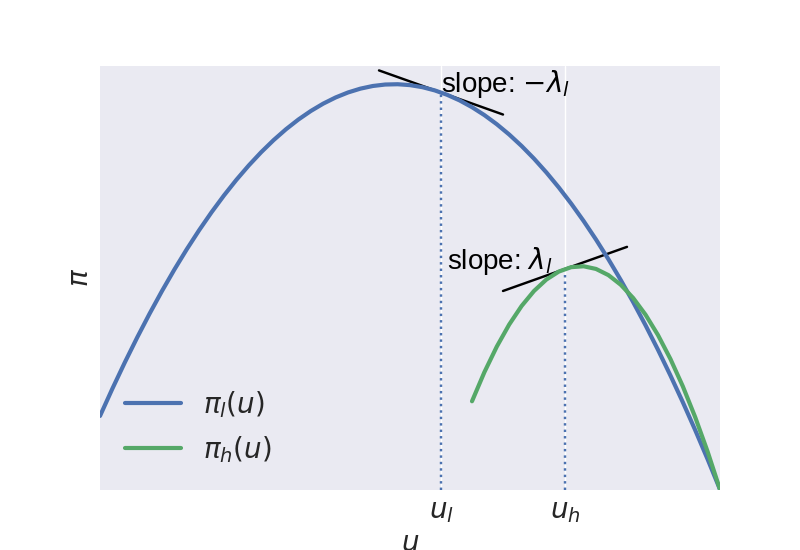
\includegraphics[width=.9\linewidth]{profitfunctions.png}
\caption{\label{fig:profitfunctions}Insurer's profits \(\pi_{l}(u),\pi_{h}(u)\) as a function of \(u\).}
\end{figure}

Given that the insurer cannot implement first best, it is willing to introduce some inefficiency which helps to separate the low from the high types. In a standard health insurance model (\citeprocitem{34}{Rothschild and Stiglitz 1976}) the \(h\) type wants to mimic the \(l\) type and the insurer introduces an inefficiency by distorting coverage of the \(l\) contract below first best coverage. In our set-up, the \(l\) type wants to mimic the \(h\) type and in response the insurer is willing to distort coverage of the \(h\) contract. This is where \(p_1>v_1\) comes in. With price above value, the first best contract would remove treatment 1 from coverage. But in second best, covering treatment 1 is the inefficiency that helps the insurer to separate the types. Hence, treatment 1 has still value for the insurer (and is willing to cover it) even though it costs more than treatment value.

In second best, the inefficiency reduces \(u_h\) below the level that would maximize \(\pi_h\). The extent to which the insurer is willing to reduce \(u_h\) depends on the elasticity \(\varepsilon_h\). The more \(h\) customers leave due to a fall in \(u_h\), the more reluctant the insurer is to introduce such a reduction.

As treatment 1 has still value for insurers at a price \(p_1 > v_1\) and they are willing to cover this treatment, the prediction is that pharmaceutical companies will charge prices above the value of their medicines. The bigger the value of \(\lambda_l v_1 \Delta \psi_1\), the higher \(p_1\) is expected to be.

\subsection{Health insurance context and summary}
\label{sec:org792322e}

In which health insurance context does the model explain excessive pricing for treatments? The main issue is selection on the insurance market. Hence, in a setting with government financed insurance (like the NHS in the UK), there is no selection on the insurance market and the model does not apply.

In the discussion of equation \eqref{eq:ICelasticities} we already note that the model does not apply with perfect competition. In that case, there are no elasticity differences between the market segments and the left hand side of equation \eqref{eq:ICelasticities} equals 0. In this sense, we need insurers with market power for the model to apply. A monopoly insurer faces selection (if health insurance is not mandatory) as well as oligopoly insurers. As long as the functions \(q_l(u_l),q_h(u_h)\) are not constants, the model applies. Insurers can distort their contracts to get a more profitable case-mix of insured. 

Finally, there are selection problems for the health insurer if it is not able to risk rate. If insurers can observe risk types and are allowed to price discriminate, the model does not apply. There are no incentive compatibility constraints with risk rating. Hence, we need either unobserved risk types or a community rating requirement. 
The appendix presents a simple analysis to illustrate that a model with only risk averse consumers (and no selection) cannot easily explain that treatments with price above value are covered by health insurance. 

Summarizing, we introduced a simple model of health insurer competition and showed that it is indeed possible for a pharmaceutical company with a patented drug to sell this at a price that exceeds treatment value. As quoted in the Introduction, some experts claim that prices for some drugs are out of proportion with the value they offer. Although this seems counter-intuitive (insurers should not cover treatments that cost more than the value they create), the model above shows that this can, in fact, happen in equilibrium.

As the private incentive to innovate is driven by \(p_1\) (profit for the company with the patent) while the social incentive is determined by \(v_1\) (value for patients), \(p_1>v_1\) implies that pharmaceutical firms have an excessive incentive to innovate: the private value of innovation exceeds the social value. The next section considers firms' incentives to target treatments at subgroups of patients.



\section{Precision medicine}
\label{sec:org80d77ad}

Now that we have seen that pricing above value can happen in equilibrium, a natural question is: for which treatments is this most likely to happen? Based on the model, we argue that this problem seems pertinent to precision medicine.

Recall from above that the marginal value for the insurer of including treatment 1 equals \(\lambda_l v_1 \Delta \psi_1 >0\). The Lagrange multiplier \(\lambda_l\) on the \(IC_l\) constraint is the same for all treatments. Hence, overpricing is likely to be bigger for treatments that have high value \(v_1\) and feature high \(\Delta \psi_1\).

The value effect is intuitive; no one is likely to worry about a treatment with a value of 10 euros. But for treatments with values around 100k, potential and damage due to over-pricing is big. As cancer treatments can potentially extend life years, treatments for such drugs are in this ball park. Without going into the literature on the value of life years (usually measured with quality adjusted life years or qaly's), a value of a healthy life year around 100k is not unreasonable (\citeprocitem{9}{Cutler 2004}).

The \(\Delta \psi_1\) term measures the difference in probability that treatment 1 is used by the \(h\) vs the \(l\) type. High \(\Delta \psi_1\) implies that the treatment is targeted at \(h\) types and hence effective at separating the types for the insurer.


One can think of two reasons why \(\Delta \psi_1\) is high for a treatment: the first is exogenous to the R\&D lab or pharmaceutical company and the second endogenous. First, it can be a matter of biology: some people suffer from diabetes and others do not. The difference between the prevalence of diabetes among high and low risk types determines \(\Delta \psi_1\) and the pharmaceutical company cannot change this.\footnote{Note the following distinction: type 2 diabetes tends to be endogenous to an individual's lifestyle but exogenous to a pharmaceutical company. Here we focus on the exogeneity with respect to the company.}

Second, a pharmaceutical R\&D lab can invest in projects that are targeted at sub-populations of patients with a disease. This captures the ``transition away from the production of `one-size-fits-all' treatments towards targeted treatments'' (\citeprocitem{11}{Dugger, Platt, and Goldstein 2018}). With precision or personalized medicine, the treatment takes the patient's underlying mechanism of the disease into account. Such targeted therapies require the co-development of diagnostic tools to identify the optimal treatment for individual patients. Biomarkers are used to define the subset of patients who benefit from the treatment. The use of biomarkers in clinical trials has increased substantially over time (\citeprocitem{6}{Chandra, Garthwaite, and Stern 2018}). According to our model this goes hand-in-hand with an increase in the number of drugs with price above value.


Advantages of precision medicine include faster development and smaller/cheaper trials because the drugs are targeted at smaller groups (\citeprocitem{6}{Chandra, Garthwaite, and Stern 2018}). Better clinical results for the sub-population of patients targeted by the treatment. Ideally, lower healthcare expenditure because of the cheaper development and the fact that the drugs are used for smaller groups. However, the last effect has not materialized as personalized medicine turns out to be very expensive.

What are the ways and incentives for pharmaceutical research labs to focus on precision medicine? Pharmaceutical companies need to select the most promising among the drug targets identified in early stages of research to pursue further (\citeprocitem{13}{Emmerich et al. 2021}; \citeprocitem{26}{Knowles and Gromo 2003}). There are two margins along which they can decide to focus on targeted drugs. The extensive margin where they prioritize targeted projects above more generic projects. The intensive margin where they decide to narrow down a given project by investing in the discovery of (more) biomarkers. This decision is partly informed by science but it turns out that there is an important role for marketing and financial directors (\citeprocitem{26}{Knowles and Gromo 2003}).

Although biomarkers ``divide the market of treatable patients into groups and clusters, thus reducing market share'' (\citeprocitem{24}{Jakka and Rossbach 2013}), this targeting can be profitable in its own right beyond the (socially) beneficial effects mentioned above. In particular, this partitioning of the market is profitable by increasing the price above treatment value; even if no extra social value is created by targeting the treatment. In this sense, there is an excessive incentive for pharmaceutical companies to target treatments with precision medicine.

To capture this idea of excessive targeting, we introduce a parameter \(\zeta\) with the properties that \(d\psi_{1h}/d\zeta <0\) and \(d\Delta \psi_1/d\zeta>0\). This we call ``high type targeting''. In words, the innovator focuses on a high type targeting strategy (increases \(\zeta\)) if its treatment will be effective for only a subset of high types (\(d\psi_{1h}/d\zeta <0\)) but for an even smaller set of low types (\(d\Delta\psi_1/d\zeta>0\)). To illustrate, consider a disease with different strains. Focusing treatment \(1\) on a particular strain that is more prevalent under high than low types, leads to a fall in \(1\)'s market share under \(h\) types --as not all \(h\) types have this strain-- and to an even bigger fall in market share under \(l\) types as they are even less likely to feature this strain. Such a drop in market share is profitable if it is compensated by an increase in \(p_1-v_1>0\) determined by \(\lambda_l v_1 \Delta \psi_1\).

The model implies that even in the (extreme) case where there is no social value to targeting at all, there is still a private incentive to do so if the increase in \(p_1\) compensates the fall in \(\psi_{1l},\psi_{1h}\). If targeting does not raise \(v_1\) nor reduce the development costs for the treatment, a social planner would not invest in targeting. But a private company would if the increase in price exceeds the fall in market share. In this sense, there is an excessive (private) incentive for the pharmaceutical sector to invest in precision medicine. The result is higher prices and higher healthcare expenditure but no increased value or life expectancy. As explained in the Introduction, this is how some experts view the developments in personalized medicine.

To the extent that the specialty pharmaceutical market and  personalized medicine are examples of high type targeting, the analysis above implies that they have contributed to the rise in treatment prices documented in the Introduction. This is also our explanation for the observation that ``payers value rarity'': prices tend to be high for (orphan) drugs with very small patient populations. If such drugs are hardly used by high types (low \(\psi_{1h}\)) and even fewer low types (high \(\Delta \psi_1\)) prices will be high as the extent to which \(p_1-v_1\) is positive is determined by \(\lambda_l \Delta \psi_1 v_1\).


\section{Policy implications}
\label{sec:orgeba2816}

This paper introduces a framework where upstream pharmaceutical companies sell drugs to a downstream health insurance market which suffers from selection problems. If the low risk type wants to buy the high risk type contract, we find that upstream firms can charge prices in excess of treatment value. Further, pharmaceutical companies have an excessive incentive to narrow their market; that is, target treatments at patient subgroups.

A couple of developments have contributed to the price increases in the pharmaceutical markets. First, the increased adoption of generic drugs has created the ``space'' for patented drugs to charge prices in excess of treatment value. Although the net value of coverage for some treatments is negative from the insured's point of view, the overall value of insurance is still positive. Second, the development to target treatments to subgroups of patients suffering from a disease also leads to upward pressure on drug prices. 

We assume that pharmaceutical companies make take-it-or-leave-it offers to insurers. We show that these offers can lead to prices above value. If, instead, pharmaceutical companies and insurers bargain over prices and insurers have some bargaining power, prices tend to be lower. The outcome can then still be a high price close to value because without insurer bargaining power prices would exceed treatment value.

The implications of our analysis for policy can be summarized as follows. First, there have been numerous recent examples of drugs being sold at very high prices. The narrative usually is that it is ``unfair'' or not ``ethical'' for pharmaceutical companies to benefit from people's health problems. We show that it is not only unfair, it may well be inefficient. By charging a price in excess of a treatment's value, R\&D incentives are distorted: (i) incentives to do R\&D can be excessive as firms earn extra profits: the private value of the innovation (\(p_1\)) exceeds the social value (\(v_1\)); (ii) firms have an excessive incentive to target their treatment to subgroups of patients: even if there is no social value to targeting, it is still privately profitable.

To reduce the excessive R\&D incentives, a government can reduce tax breaks for R\&D in the pharmaceutical sector and increase the industry's financial contribution to research by (public) universities both for fundamental research and for running trials to test new treatments. Further, the government can consider introducing price caps; for instance, in the form of not approving treatments for insurance coverage if the price per qaly (quality adjusted life year) gained is too high. This helps to keep the healthcare system affordable and reduces excessive R\&D incentives. As shown, relying on market forces to keep prices low does not work for an upstream sector selling to a downstream market with selection problems.

Finally, assuming that consumers stop buying insurance in case the expected value of the insurance plan is lower than the premium, treatment prices can be reduced by creating a separate insurance market for patented treatments. The separation would be similar to having basic and supplementary insurance markets as some countries have; but here there would be insurance for patented drugs and separate insurance for treatments  where the patent has run out (like generic drugs). The latter insurance would cover all generic drugs which yield high patient utility compared to their cost. This leaves less rents for patented treatments on their insurance market segment to appropriate by charging a price above treatment value. Such a segmentation of the health insurance market helps to reduce treatment prices and healthcare expenditure.

\section{Bibliography}
\label{sec:orgf399dbc}

\hypertarget{citeproc_bib_item_1}{Atherly, Adam, Bryan E. Dowd, and Roger Feldman. 2004. “The Effect of Benefits, Premiums, and Health Risk on Health Plan Choice in the Medicare Program.” \textit{Health Services Research} 39 (4p1): 847–64.}

\hypertarget{citeproc_bib_item_2}{Auerbach, David, and Sabina Ohri. 2006. “Price and the Demand for Nongroup Health Insurance.” \textit{INQUIRY: The Journal of Health Care Organization, Provision, and Financing} 43 (2): 122–34.}

\hypertarget{citeproc_bib_item_3}{Beaulieu, Nancy Dean. 2002. “Quality Information and Consumer Health Plan Choices.” \textit{Journal of Health Economics} 21 (1): 43–63.}

\hypertarget{citeproc_bib_item_4}{Cavalli, Franco. 2013. “An Appeal to World Leaders: Stop Cancer Now.” \textit{The Lancet} 381 (9865): 425–26.}

\hypertarget{citeproc_bib_item_5}{Chandra, Amitabh, Evan Flack, and Ziad Obermeyer. 2021. “The Health Costs of Cost-Sharing,” February. National Bureau of Economic Research. doi:\href{https://doi.org/10.3386/w28439}{10.3386/w28439}.}

\hypertarget{citeproc_bib_item_6}{Chandra, Amitabh, Craig Garthwaite, and Ariel Dora Stern. 2018. “Characterizing the Drug Development Pipeline for Precision Medicines.” In \textit{Economic Dimensions of Personalized and Precision Medicine}, 115–57. University of Chicago Press.}

\hypertarget{citeproc_bib_item_7}{Cohn, J. 2007. \textit{Sick: The Untold Story of America’s Health Care Crisis–and the People Who Pay the Price}. Harper Perennial.}

\hypertarget{citeproc_bib_item_8}{Costa, Joan, and Jaume Garcia. 2003. “Demand for Private Health Insurance: How Important Is the Quality Gap?” \textit{Health Economics} 12 (7). Wiley: 587–99. doi:\href{https://doi.org/10.1002/hec.756}{10.1002/hec.756}.}

\hypertarget{citeproc_bib_item_9}{Cutler, D.M. 2004. \textit{Your Money or Your Life: Strong Medicine for America’s Healthcare System}. Oxford University Press.}

\hypertarget{citeproc_bib_item_10}{Doble, Brett. 2016. “Budget Impact and Cost-Effectiveness: Can We Afford Precision Medicine in Oncology?” \textit{Scandinavian Journal of Clinical and Laboratory Investigation} 76 (sup245). Taylor \& Francis: S6–S11.}

\hypertarget{citeproc_bib_item_11}{Dugger, S.A., A. Platt, and D.B. Goldstein. 2018. “Drug Development in the Era of Precision Medicine.” \textit{Nature Reviews Drug Discovery} 17: 183–96. doi:\href{https://doi.org/10.1038/nrd.2017.226}{10.1038/nrd.2017.226}.}

\hypertarget{citeproc_bib_item_12}{Einav, Liran, and Amy Finkelstein. 2011. “Selection in Insurance Markets : Theory and Empirics in Pictures.” \textit{Journal of Economic Perspectives} 25 (1): 115–38.}

\hypertarget{citeproc_bib_item_13}{Emmerich, C.H., L.M. Gamboa, M.C.J. Hofmann, M. Bonin-Andresen, O. Arbach, P. Schendel, B. Gerlach, et al. 2021. “Improving Target Assessment in Biomedical Research: The GOT-IT Recommendations.” \textit{Nature Reviews Drug Discovery} 20: 64–81. doi:\href{https://doi.org/10.1038/s41573-020-0087-3}{10.1038/s41573-020-0087-3}.}

\hypertarget{citeproc_bib_item_14}{Finkelstein, A., and K. McGarry. 2006. “Multiple Dimensions of Private Information: Evidence from the Long-Term Care Insurance Market.” \textit{The American Economic Review} 96 (4). JSTOR: 938–58.}

\hypertarget{citeproc_bib_item_15}{Frijters, P., J.P. Haisken-DeNew, and M.A. Shields. 2005. “The Causal Effect of Income on Health: Evidence from German Reunification.” \textit{Journal of Health Economics} 24 (5). Elsevier: 997–1017.}

\hypertarget{citeproc_bib_item_16}{Garattini, Livio, Alessandro Curto, and Nick Freemantle. 2015. “Personalized Medicine and Economic Evaluation in Oncology: All Theory and No Practice?” \textit{Expert Review of Pharmacoeconomics \& Outcomes Research} 15 (5). Taylor \& Francis: 733–38.}

\hypertarget{citeproc_bib_item_17}{Garrison, Jr. L.P., and A. Towse. 2017. “Value-Based Pricing and Reimbursement in Personalised Healthcare: Introduction to the Basic Health Economics.” \textit{Journal of Personalized Medicine} 7 (3).}

\hypertarget{citeproc_bib_item_18}{Gaynor, Martin, Kate Ho, and Robert J. Town. 2015. “The Industrial Organization of Health-Care Markets.” \textit{Journal of Economic Literature} 53 (2): 235–84.}

\hypertarget{citeproc_bib_item_19}{Gravelle, H., and M. Sutton. 2009. “Income, Relative Income, and Self-Reported Health in Britain 1979-2000.” \textit{Health Economics} 18 (2): 125–45.}

\hypertarget{citeproc_bib_item_20}{Handel, Benjamin, Jonathan Kolstad, Thomas Minten, and Johannes Spinnewijn. 2020. “The Social Determinants of Choice Quality: Evidence from Health Insurance in the Netherlands,” September. National Bureau of Economic Research. doi:\href{https://doi.org/10.3386/w27785}{10.3386/w27785}.}

\hypertarget{citeproc_bib_item_21}{Handel, Benjamin R., and Jonathan T. Kolstad. 2015. “Health Insurance for ‘Humans’: Information Frictions, Plan Choice, and Consumer Welfare.” \textit{American Economic Review} 105 (8): 2449–2500.}

\hypertarget{citeproc_bib_item_22}{Ho, Kate, Joseph Hogan, and Fiona Scott Morton. 2017. “The Impact of Consumer Inattention on Insurer Pricing in the Medicare Part D Program.” \textit{The RAND Journal of Economics} 48 (4): 877–905.}

\hypertarget{citeproc_bib_item_23}{Howard, David H., Peter B. Bach, Ernst R. Berndt, and Rena M. Conti. 2015. “Pricing in the Market for Anticancer Drugs.” \textit{Journal of Economic Perspectives} 29 (1): 139–62. doi:\href{https://doi.org/10.1257/jep.29.1.139}{10.1257/jep.29.1.139}.}

\hypertarget{citeproc_bib_item_24}{Jakka, Sairamesh, and Michael Rossbach. 2013. “An Economic Perspective on Personalized Medicine.” \textit{The HUGO Journal} 7 (1): 1.}

\hypertarget{citeproc_bib_item_25}{Kamphorst, Jurjen, and Vladimir A. Karamychev. 2021. “Going through the Roof: On Prices for Drugs Sold through Insurance.” Erasmus University Rotterdam.}

\hypertarget{citeproc_bib_item_26}{Knowles, J., and G. Gromo. 2003. “Target Selection in Drug Discovery.” \textit{Nature Reviews Drug Discovery} 2: 63–69.}

\hypertarget{citeproc_bib_item_27}{Lewis, Tracy R, and David E.M Sappington. 1989. “Countervailing Incentives in Agency Problems.” \textit{Journal of Economic Theory} 49 (2): 294–313.}

\hypertarget{citeproc_bib_item_28}{Mahoney, Neale, and E. Glen Weyl. 2017. “Imperfect Competition in Selection Markets.” \textit{The Review of Economics and Statistics} 99 (4): 637–51.}

\hypertarget{citeproc_bib_item_29}{Medic, G., D. Korchagina, K.E. Young, M. Toumi, M.J. Postma, M. Wille, and M. Hemels. 2017. “Do Payers Value Rarity? an Analysis of the Relationship between Disease Rarity and Orphan Drug Prices in Europe.” \textit{Journal of Market Access and Health Policy} 5.}

\hypertarget{citeproc_bib_item_30}{Messori, Andrea, Americo Cicchetti, and Luigi Patregani. 2010. “Relating Price Determination to Disease Prevalence.” \textit{BMJ} 341. BMJ Publishing Group Ltd. doi:\href{https://doi.org/10.1136/bmj.c4615}{10.1136/bmj.c4615}.}

\hypertarget{citeproc_bib_item_31}{Munkin, M.K., and P.K. Trivedi. 2010. “Disentangling Incentives Effects of Insurance Coverage from Adverse Selection in the Case of Drug Expenditure: A Finite Mixture Approach.” \textit{Health Economics} 19 (9): 1093–1108.}

\hypertarget{citeproc_bib_item_32}{Nyman, John A. 1999. “The Value of Health Insurance: The Access Motive.” \textit{Journal of Health Economics} 18 (2): 141–52.}

\hypertarget{citeproc_bib_item_33}{Parente, Stephen T., Roger Feldman, and Jon B. Christianson. 2004. “Employee Choice of Consumer-Driven Health Insurance in a Multiplan, Multiproduct Setting.” \textit{Health Services Research} 39 (4p2): 1091–1112.}

\hypertarget{citeproc_bib_item_34}{Rothschild, M., and J. Stiglitz. 1976. “Equilibrium in Competitive Insurance Markets: An Essay on the Economics of Imperfect Information.” \textit{The Quarterly Journal of Economics} 90 (4): 629–49.}

\hypertarget{citeproc_bib_item_35}{Royalty, Anne Beeson, and Neil Solomon. 1999. “Health Plan Choice: Price Elasticities in a Managed Competition Setting.” \textit{The Journal of Human Resources} 34 (1). [University of Wisconsin Press, Board of Regents of the University of Wisconsin System]: 1–41.}

\hypertarget{citeproc_bib_item_36}{Saltzman, Evan. 2019. “Demand for Health Insurance: Evidence from the California and Washington ACA Exchanges.” \textit{Journal of Health Economics} 63: 197–222. doi:\url{https://doi.org/https://doi.org/10.1016/j.jhealeco.2018.11.004}.}

\hypertarget{citeproc_bib_item_37}{Schoen, Cathy, Sara R Collins, Jennifer L Kriss, and Michelle M Doty. 2008. \href{https://www.ncbi.nlm.nih.gov/pubmed/18544591}{“How Many Are Underinsured? Trends among U.S. Adults, 2003 and 2007.}” \textit{Health Affairs (Project Hope)} 27 (4): 298–309.}

\hypertarget{citeproc_bib_item_38}{Schoen, C, R Osborn, D Squires, M M Doty, R Pierson, and S Applebaum. 2010. \href{https://www.ncbi.nlm.nih.gov/pubmed/21088012}{“How health insurance design affects access to care and costs, by income, in eleven countries.}” \textit{Health Affairs} 29 (12): 1–12.}

\hypertarget{citeproc_bib_item_39}{Schokkaert, Erik, and Carine van de Voorde. 2011. “Chapter 15 - User Charges.” In \textit{Oxford Handbook of Health Economics}, edited by S. Glied and P. Smith, 329–53. Oxford University Press.}

\hypertarget{citeproc_bib_item_40}{Strombom, Bruce A, Thomas C Buchmueller, and Paul J Feldstein. 2002. “Switching Costs, Price Sensitivity and Health Plan Choice.” \textit{Journal of Health Economics} 21 (1): 89–116.}

\hypertarget{citeproc_bib_item_41}{Tirole, Jean. 1988. \textit{The Theory of Industrial Organization}. MIT Press.}\bigskip



\newpage
\appendix



\setcounter{table}{0}
\renewcommand{\thetable}{\thesection\arabic{table}}


\section{Model with risk aversion}
\label{sec:org80d6772}

In this appendix we consider a model with only risk aversion to understand what the selection model used in the main text adds to a risk aversion model. The idea is that a model with risk aversion (only) can also explain that treatment producers charge a price above the value of their treatment. Intuitively, insurance creates a surplus for the insurer-provider combination that both parties can bargain over. If the treatment supplier has sufficient bargaining power, this can lead to a price above treatment value.

The point of this section is to illustrate that: (i) it is not obvious that a model with a risk averse agent can generate this result and (ii) if it does lead to \(p>v\), it does so mainly for treatments that are used by many people. In the Introduction we showed that the evidence for over-pricing is in markets for (very) small patient populations e.g. due to precision medicine.

Consider a simple model with two states of the world: an agent falls ill and needs treatment (probability \(\psi \in \langle0,1\rangle\)) and the agent is healthy (probability \(1-\psi\)). In the bad state of the world, the agent's utility is given by \(u_b(.)\) and in the good state of the world by \(u_g(.)\), where we assume increasing and concave utility in each state of the world: \(u'_i > 0, u''_i <0, i=g,b\).

If the agent receives treatment in the bad state her utility equals \(u_b(y+v)\) where \(y\) denotes the agent's income that is spent on consumption and \(v\) the (consumption) value of the treatment. We assume that the treatment has no value in the good state of the world. If there is no insurance, the agent would buy the treatment if and only if \(u_b(y+v-p) \geq u_b(y)\) where \(p\) denotes the (uninsured) price of the treatment. Clearly, this implies that an uninsured only buys treatment if \(p \le v\).

Let \(x \in [0,1]\) denote the fraction of treatment covered by insurance. We want to see whether a consumer chooses \(x=1\) if \(p>v\). That is, a risk averse consumer buys insurance for a treatment with a price in excess of the treatment's value. We assume perfect competition in the health insurance market: \(\sigma = \psi x p\). Then utility can be written as:
\begin{equation}
\label{eq:utility}
U(x) = (1-\psi) u_g(y-\sigma) + \psi u_b (y+xv-\sigma)
\end{equation}
The first derivative with respect to \(x\) can be written as
\begin{equation}
\label{eq:DutilityDx}
\frac{dU}{dx}=-(1-\psi)u'_g(y-\sigma) \psi p + \psi u'_b(y+xv-\sigma)(v-\psi p)
\end{equation}
To see whether the agent is willing to buy insurance, consider \(dU/dx\) evaluated at \(x=0\). In words, starting from no insurance, would the agent be willing to increase \(x\) (ultimately to \(x=1\)):
\begin{equation}
\label{eq:DutilityDxAt0}
\left. \frac{dU}{dx} \right|_{x=0} = \psi u'_g(y) \left( \left(\frac{u'_b}{u'_g} -1 \right) (1-\psi)p + \frac{u'_b}{u'_g} (v-p)  \right)
\end{equation}
A natural assumption seems to be that \(u'_g(y) \ge u'_b(y)\): the marginal utility of consumption is higher when you are healthy than when you are ill. You can enjoy consumption more when you can travel, visit friends, go skiing than when you are in hospital or at home lying in bed all day. Then the last equation makes clear that \(p>v\) implies \(dU/dx < 0\) at \(x=0\). In words, the consumer does not want to buy health insurance if the treatment features \(p>v\).

This is not to argue that it is impossible to write down a model where risk aversion leads to \(p>v\). We only illustrate that it is not obvious that risk aversion can explain pricing above value.

If we are willing to assume that \(u'_b > u'_g\), we can have \(dU/dx >0\) but the equation shows that \(dU/dx > 0\) is small for treatments with \(\psi\) close to zero. That is, treatments that are only used by small groups of patients are unlikely to be able to claim much of the joint surplus created by risk aversion. But as shown in the Introduction it is for these (very) rare diseases that we see the most ``outrageous'' prices. A model based on risk aversion cannot explain this observation that payers value rarity. Finally, there is no incentive for pharmaceutical firms to reduce \(\psi\) through precision medicine unless this would increase treatment value or reduce costs (which we do not tend to observe in the real world). Therefore, we find the model based on selection in the main text more useful for this analysis than a model based on risk-aversion.
\end{document}